\chapter{Grundlagen}
Auf der Basis einer wissenschaftlichen Literaturrecherche werden im Folgenden die benötigten Grundlagen für den weiteren Verlauf dieser Arbeit aufgezeigt:

\section{Einführung in cFront} \label{cFront-exp}
Die Abteilung \textit{cGroup Solutions} beschäftigt sich mit der Entwicklung von Anwendungen zur Unterstützung von Airlines und Flughäfen. Dazu gehört u.a. auch das Produkt \textit{cFront}. Ziel dieses Produkts ist es, eine gemeinsame Nutzung der digitalen Infrastruktur an Flughäfen für Airlines zu ermöglichen.
Es wird dabei an Terminals verschiedener Flughäfen eingesetzt wird. So können beispielsweise die Passagier- und Flugabfertigung verschiedener Airlines über die gleiche Hardware erfolgen. \textit{cFront} bietet somit eine standardisierte Schnittstelle zu den individuellen Applikationen der verschiedenen Airlines.

\begin{figure}[h]
	\centering 
	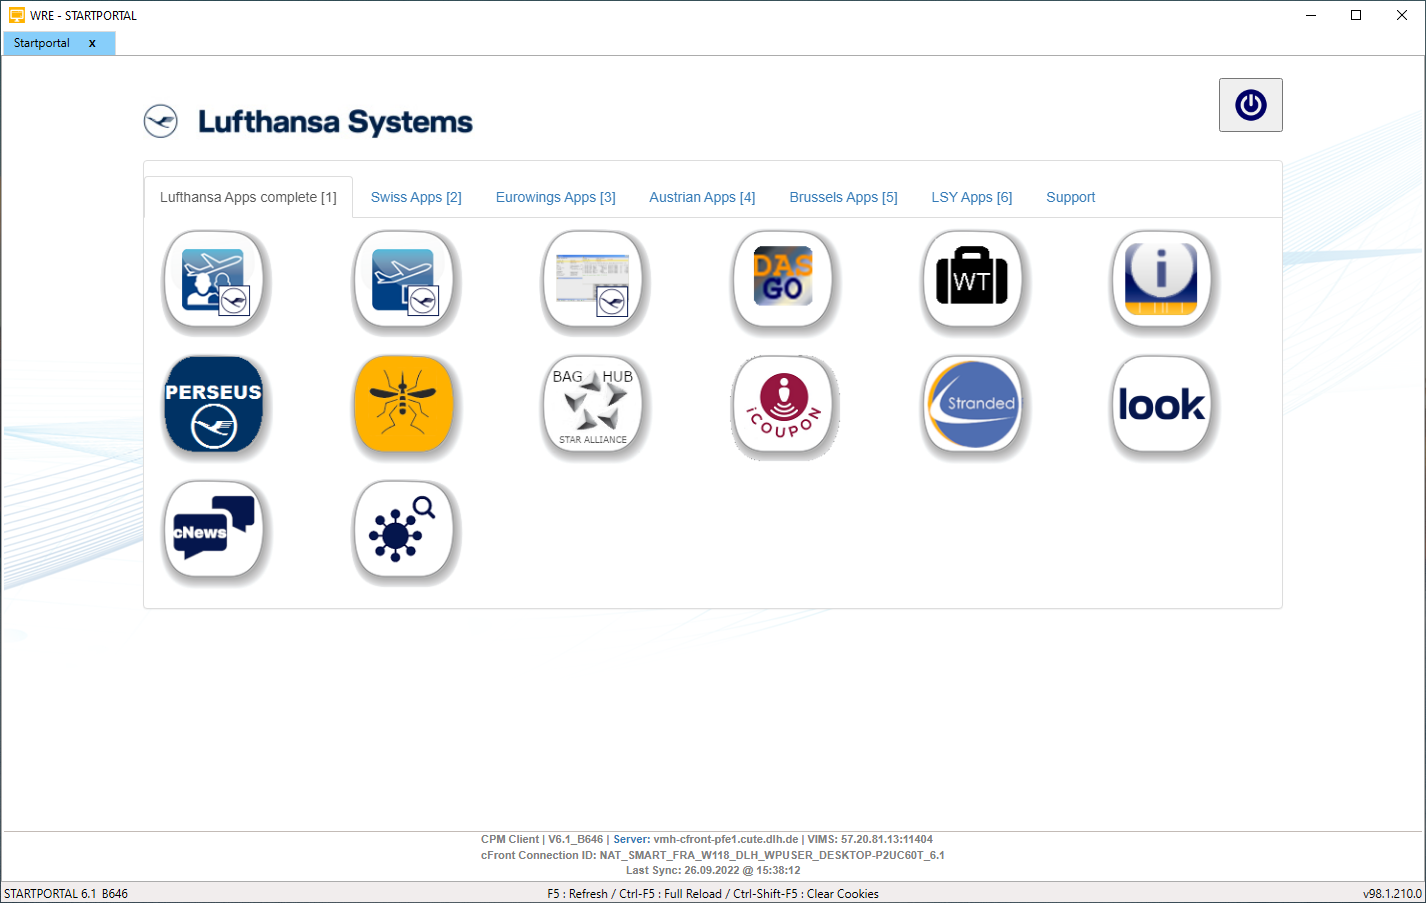
\includegraphics[width=1\textwidth]{img/abbildungen/MicrosoftTeams-image (3).png}
	\captionsetup{format=hang}
	\caption{cFront Startportal} \label{cFront}
\end{figure}

Es agiert dabei als Interface für mehrere Anwendung und ermöglicht es den Kunden, diese Anwendungen zu starten. Welche Anwendungen sichtbar sind, kann je nach Kunde individuell konfiguriert werden. Ein Beispiel für ein solches Interface wird in \textbf{\ref{cFront}} dargestellt.
Die verschiedenen Icons im mittleren Bereich der Abbildungen stellen die individuellen Applikationen der jeweiligen Airline da. Bei der Abbildung handelt es sich lediglich um Beispieldaten und keine reale Konfiguration.


\section{CIA-Triade}

Die CIA-Triade gehört zu den wichtigsten Darstellungen von Sicherheitszielen innerhalb der Informationssicherheit. Sie beschreibt die drei Schutzziele \textit{Confidentiality} (Vertraulichkeit), \textit{Integrity} (Integrität) und \textit{Availability} (Verfügbarkeit). Im Folgenden werden diese kurz beschrieben:

\begin{figure}[h]
	\centering 
	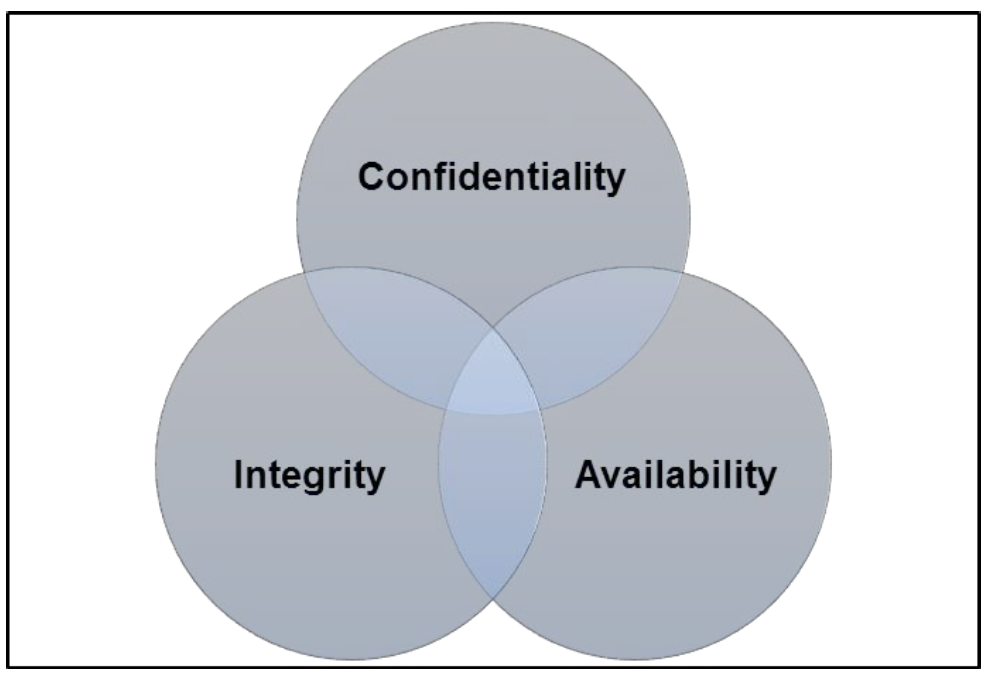
\includegraphics[width=0.5
    \textwidth]{img/abbildungen/CIA-Triad.png}
	\captionsetup{format=hang}
	\caption{CIA-Triad} \label{CIA-Triad}
\end{figure}

\paragraph*{Confidentiality} 
Die Vertraulichkeit gehört zu den wichtigsten Schutzzielen in der Informationssicherheit \cite{samonas2014cia}. Das Wort \textit{Confidentiality} kommt vom lateinischen Wort \textit{confidere} und bedeutet \textit{vertrauen} \cite{pons} \cite{samonas2014cia}. Das Schutzziel der Vertraulichkeit besagt, dass Informationen und Daten so geschützt sein müssen, dass diese nur von autorisierten Personen und für autorisierte Zwecke genutzt werden können \cite{samonas2014cia}. 
Dies beinhaltet beispielsweise Einschränkungen des Zugriffs auf Informationen und Daten, um die Privatsspähre und persönliches Eigentum zu schützen \cite{samonas2014cia}. Aber auch Verschlüsselungen, eine sichere Authentifizierung und Sicherheitsprotokolle können zur Gewährleistung der Vertraulichkeit beitragen \cite{agarwal2011security}.
Aufgrund der steigenden Wichtigkeit von wirtschaftlichen Aspekten hat die Vertraulichkeit im Vergleich zu früher an Bedeutung verloren \cite{samonas2014cia}. Häufig werden Schutzziele vernachlässigst, um im Gegenzug eine erhöhte Benutzerfreundlichkeit oder Wirtschaftlichkeit zu erreichen.

\paragraph*{Integrity}  
Das Wort \textit{Integrity} leitet sich vom lateinischen Wort \textit{tangere} ab und bedeutet so viel wie \textit{berühren} \cite{pons}. Durch die Vorsilbe \textit{In-} soll eine gegenteilige Bedeutung  im Sinne von \textit{Unberührbarkeit} entstehen \cite{samonas2014cia}. 
Die Integrität soll somit garantieren, dass Daten nicht verändert werden können, ohne dass dies bemerkt wird \cite{agarwal2011security}. Schickt ein Sender $S$ beispielsweise eine Nachricht an einen Empfänger $E$, so soll die Nachricht identisch beim Empfänger $E$ ankommen, wie sie vom Sender $S$ gesendet wurde \cite{agarwal2011security}.
Umsetzungsmöglichkeiten die Integrität zu schützen beinhalten Maßnahmen wie beispielsweise das Verwenden einer Firewall, eines \ac{IDS} oder auch digitale Signaturen \cite{agarwal2011security}.

\paragraph*{Availability}
Das Wort Availability leitet sich vom lateinischen \textit{valere} ab und bedeutet so viel wie \textit{kräftig sein}. Die Verfügbarkeit bezieht sich somit auf einen zeitnahen und und zuverlässigen Zugriff auf Informationen und Daten \cite{samonas2014cia}. Zuverlässig bedeutet dabei auch, dass ein Zugriff möglichst ohne Unterbrechungen und unabhängig vom Standort möglich ist \cite{agarwal2011security}.
Verfügbarkeit kann beispielsweise durch Netzwerksicherheit (z.B. Schutz vor \ac{DDoS}) oder Fehlertoleranz (z.B. durch Limitierung von Authentifizierungsversuchen) gewährleistet werden \cite{agarwal2011security}.

Ein wichtiger Aspekt der Schutzziele ist, dass diese nicht unabhängig voneinander betrachtet werden dürfen. Vielmehr handelt es sich, um ein Zusammenspiel der verschiedenen Schutzziele (siehe \textbf{\ref{CIA-Triad}}). So kann eine einzelne Sicherheitsmaßnahme beispielsweise mehrere Schutzziele schützen. Ebenfalls lassen sich weitere Schutzziele aus den drei bestehenden ableiten. Häufig werden erweiterte Schutzziele wie beispielsweise die \textit{Authenticity} (Authentizität) oder die \textit{Non-repudiation} (Nicht-Abstreitbarkeit) \cite{samonas2014cia} definiert. Diese können dabei zumeist von einem oder mehreren Schutzzielen der CIA-Triade abgeleitet werden. Die folgende Grafik zeigt beispielhaft einige erweiterte Schutzziele und deren Bezug zu der CIA-Triade:

\begin{figure}[h]
	\centering 
	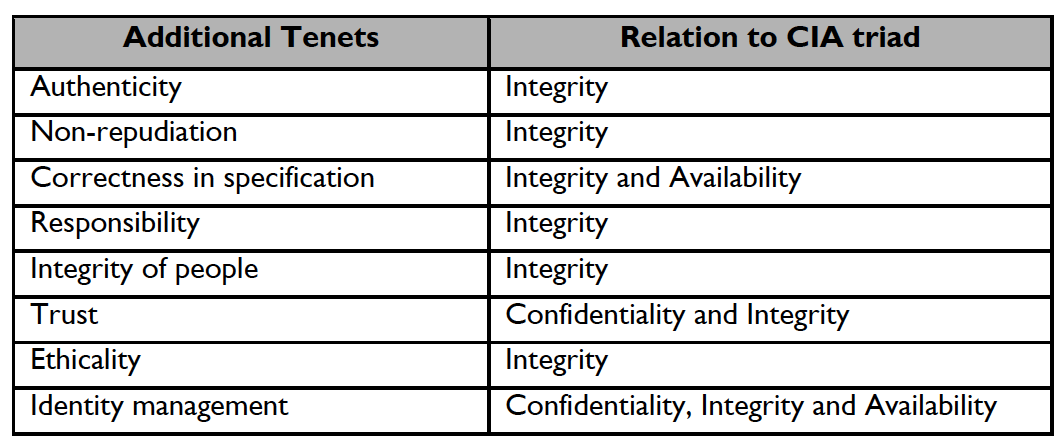
\includegraphics[width=0.8\textwidth]{img/abbildungen/Schutzziele.png}
	\captionsetup{format=hang}
	\caption{Erweiterte Schutzziele \cite{samonas2014cia}} \label{Schutzziele}
\end{figure}



\section{Arten der Authentifizierung}

Die Authentifizerung dient häufig als erste Verteidigungslinie von Systemen \cite{boonkrong2012security}. Sie gilt dabei als erweitertes Schutzziel und ist eine der wichtigsten Schutzmaßnahmen für technische Systeme. Sie übernimmt die Kontrolle über die Zugänge von Systemen und überprüft, welche Identität autorisiert ist, diese zu nutzen. In der Fachliteratur wird häufig zwischen drei verschiedenen Arten der Authentifizierung unterschieden, welche umgangssprachlich auch als \textit{Faktoren} bekannt sind. Diese sollen im Folgenden beschrieben werden:

\begin{figure}[h]
	\centering 
	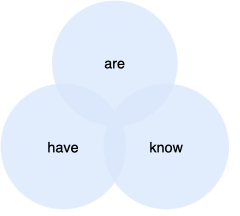
\includegraphics[width=0.4\textwidth]{img/abbildungen/factors.png}
	\captionsetup{format=hang}
	\caption{Faktoren der Authentifizierung}
\end{figure}

\paragraph*{Something you know:}
Die meistgenutzte Art der Authentifizierung basiert auf dem Wissen des Nutzers. Diese Methode nutzt Informationen - welche nur dem Nutzer bekannt sind - und bestätigt so seine Identität \cite{boonkrong2012security}. Das bekannteste Verfahren ist dabei die Nutzung von Passwörtern, welche nur dem Nutzer bekannt sind. Weitere Verfahren dieser Kategorie sind allerdings auch Sicherheitsfragen. Diese werden initial vom Nutzer beantwortet und im weiteren Verlauf zur Authentifizierung abgefragt.

\paragraph*{Something you have:}
Diese Art der Authentifizierung nutzt physische Objekte, um die Identität eines Nutzers zu verifizieren. Es handelt sich dabei um Objekte die sich lediglich im Besitz des Nutzers befinden \cite{boonkrong2012security}. Mögliche Beispiele für diese Methode sind Smartcards, welche an physische Zutrittskontrollen gehalten werden müssen oder Hardware Tokens, die für die Anmeldung an Systemen genutzt werden.

\paragraph*{Something you are:}
Diese Art der Authentifizierung basiert auf der Inhärenz. Das bedeutet, dass zur Verifizierung der Identität eines Nutzers biometrische Merkmale verwendet werden \cite{boonkrong2012security}. Dazu gehören u.a. Fingerabdrücke, Geischtserkennungen und Iris-Scans. Diese Methode hat sich besonders im Bereich der mobilen Systeme etabliert, so bietet Apple bei seinen Smartphones beispielsweise eine Authentifizierung per Fingerabdruck (\textit{Touch ID}) oder Gesichtserkennung (\textit{Face ID}) an. Aber auch Microsoft bietet eine Authentifizierung mittels biometrischer Daten an (\textit{Windows Hello} und \textit{Hello for Business}). Diese eignet sich nicht nur für mobile Endgeräte.

Ähnlich zu der CIA-Triade lassen sich auch hier weitere Faktoren ergänzen oder ableiten. Ein weiterer Faktor ist beispielsweise \textit{something you produce} \cite{boonkrong2012security}. Diese Art der Authentifizierung leitet sich teilweise von dem Faktor \textit{something you are} ab. Sie nutzt beispielsweise die Stimme des Nutzers oder seine (digitale) Unterschrift, um seine Identität zu verifizieren \cite{boonkrong2012security}. 

Die verschiedenen Arten der Authentifizierung spielen auch bei der Unterscheidung zwischen einer \ac{SFA} und einer  \ac{MFA} eine wichtige Rolle. Wird eine einzelner Faktor genutzt, so bezeichnet man dies als \ac{SFA}. Werden mehrere Faktoren genutzt handelt es sich um eine \ac{MFA}.

\section{Passwortbasierte Authentifizierung}\label{pw-auth}

    Die heutzutage am häufigsten genutzte Methode zur Authentifizierung ist die passwortbasierte Authentifizierung \cite{chanda2016password} \cite{boonkrong2012security} \cite{yildirim2019encouraging}. Diese basiert auf dem Faktor \textit{something you know}, also auf dem Wissen der Nutzer. Zumeist handelt es sich um alphanumerische Passwörter, welche aus einer Kombination von Groß- und Kleinbuchstaben, Zahlen und Sonderzeichen bestehen \cite{chanda2016password}. Die Sicherheit informationstechnischer Systeme ist somit abhängig von der Sicherheit der genutzten Passwörter \cite{boonkrong2012security}. Trotz ihrer weitreichenden Verbreitung gelten Passwörter als eine der größten Sicherheitsrisiken für Systeme, da sie vile Schwachstellen und Angriffsvektoren bieten \cite{yildirim2019encouraging} \cite{farke2020you}. Laut einer Studie von \textit{Verizon} basierten 2017 81\% der Hackerangriffe auf der Kompromittierung von Passörtern \cite{barbosa2021provable} \cite{verizon2017}. Eine weitere Studie zeigt auf, dass 2017 Phishing E-Mails die Angriffsmethode darstellte \cite{Symantec} \cite{barbosa2021provable}. Diese sind darauf ausgelegt an Passwörter von Nutzern zu gelangen. Eine Vielzahl von großen Unternehmen wurden bereits Opfer von der Veröffentlichung von Passwörtern, obwohl ein hoher Aufwand betrieben wird, um diese zu schützen \cite{boonkrong2012security}. Da sich die Enthüllung der Passwörter allerdings als Angriffsziel bei Angreifern etabliert hat, ist selbst ein hoher Aufwand nicht mehr immer ausreichend, um jene zu schützen \cite{boonkrong2012security}. Der entstehende Schaden ist immens, da es sich um einen hohen Geldwert, aber u.a. auch um einen Reputationsschaden handeln kann. Trotz der bekannten Schwachstellen und bereits entwickelten alternativen Ansätzen, bleibt das Passwort weiterhin genutzt \cite{ives2004domino}. Dies liegt insbesondere an der Einfachheit und dem geringen Aufwand, welche die Nutzung von Passwörtern mit sich bringt \cite{yildirim2019encouraging}.

    Passwörter können durch verschiedene Arten von Angriffen kompromittiert werden. So können Angreifer beispielsweise Zugriff auf die Datenbank erhalten, in welcher die Passwörter gespeicghert werden, aber auch auf persönlicher Ebene können Passörter erlangt werden. Dabei spielt das sog. Social Engineering eine große Rolle. Durch Shoulder Surfing können Angreifer versuchen Nutzern beim Passwort eintippen zuschauen. Mit Hilfe von Dumpster Diving können beispielsweise aufgeschriebene Passwörter erlangt werden. Zu den häufigsten Social Engineering Angriffen gehören allerdings die bereits beschriebenen Phishing Mails. Auf technischer Ebene ist ebenfalls ein Einsatz von Keyloggern möglich, welche alle Tastendrücke des Nutzers speichert. Ein häufig gewähltes und sehr effektives Mittel bei schlechten Passwörtern sind allerdings Brute-Force- und Dictionary-Angriffe. Diese kompromittieren Passwörter durch das stupide Ausprobieren aller möglichen Kombinationen oder die Nutzung von Tabellen, welche die meistgenutzten Passwörter beinhalten \cite{chanda2016password} \cite{morii2017research}.

    Um Passwörter resistenter gegen Brute-Force-Angriffe zu gestalten, kann eine Erweiterung des Zeichenraums oder der Passwort-Länge genutzt werden. So wird die mögliche Anzahl an Kombinationen des Passworts erhöht. Je mehr mögliche Kombinationen es gibt, desto schwieriger wird es Passwörter durch Erraten zu komprommittieren \cite{chanda2016password}. Wichtig ist hierbei, dass die Erweiterung der Passwortlänge deutlich effektiver ist als die Erweiterung des Zeichenraums. Betrachtet man die Anzahl aller Elemente des Zeichenraums $Z$ und die Passwortlänge $L$, so wird die Komplexität eines Passwortes durch $Z^L$ abgebildet. Während die Erweiterung der Passwortlänge ein exponentielles Wachstum aufweist, steigt bei einer Erweiterung des Zeichenraums die Steigung lediglich linear. Die Effektivität längerer Passwörter wird ebenfalls in \textbf{\ref{EntropyvsLength}} und \textbf{\ref{timetobreak}} dargestellt. \textbf{\ref{EntropyvsLength}} stellt die Entropie von Passwörtern in Abhängigkeit ihrer Länge dar. Dabei werden ebenfalls verschieden große Zeichenräume betrachtet. Es wird deutlich, dass selbst eine hohe Differenz des Zeichenraumes lediglich einen geringen Einfluss auf die Entropie hat. Unabhängig vom Zeichenraum aber dennoch eine hohe Entropie durch ein größere Länge möglich ist. \textbf{\ref{timetobreak}} stellt die benötigte Zeit zum Brechen von Passwörtern in Abhängigkeit zu ihrer Länge dar. Bei beiden Varianten handelt es sich um eine zu kurze Länge eines Passwortes, allerdings ist der signifikante Unterschied durch die Erweiterung der Passwortlänge um eins deutlich erkennbar.

    \begin{figure}[h]
        \centering 
        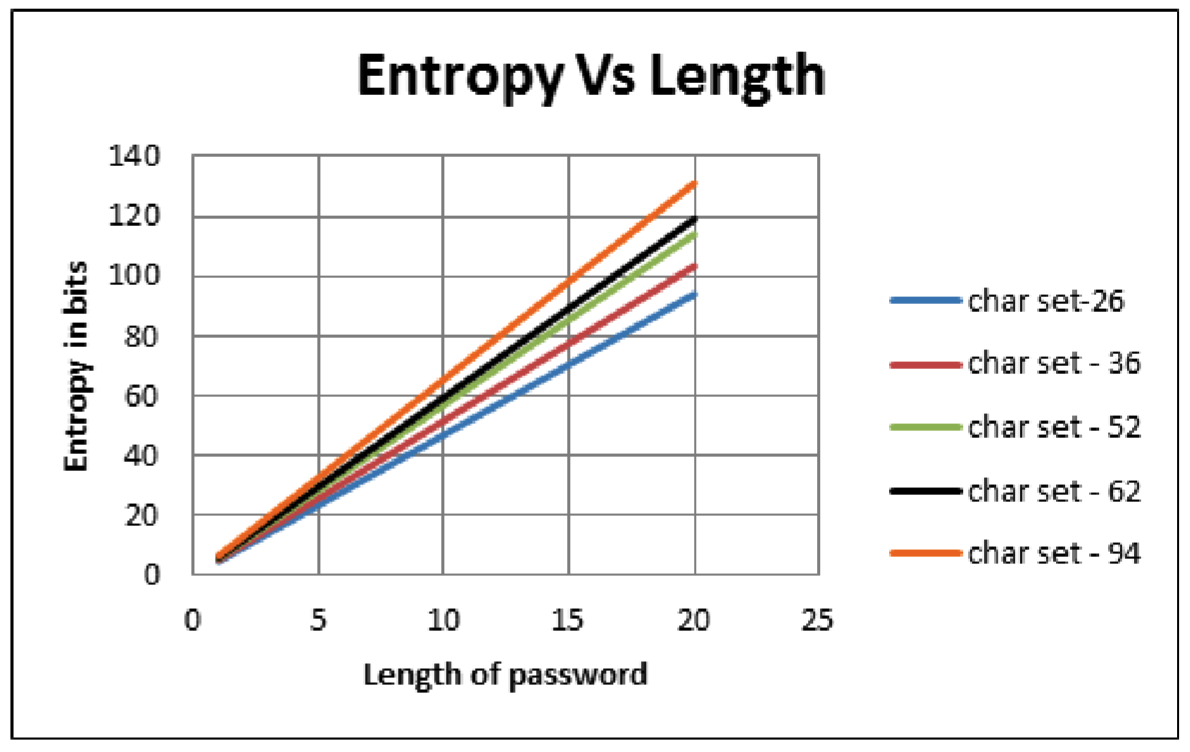
\includegraphics[width=0.7\textwidth]{img/abbildungen/entropy-length.png}
        \captionsetup{format=hang}
        \caption{Entropie in Abhängigkiet der Passwortlänge} \label{EntropyvsLength}
    \end{figure}
    
    \begin{figure}[H]
        \centering 
        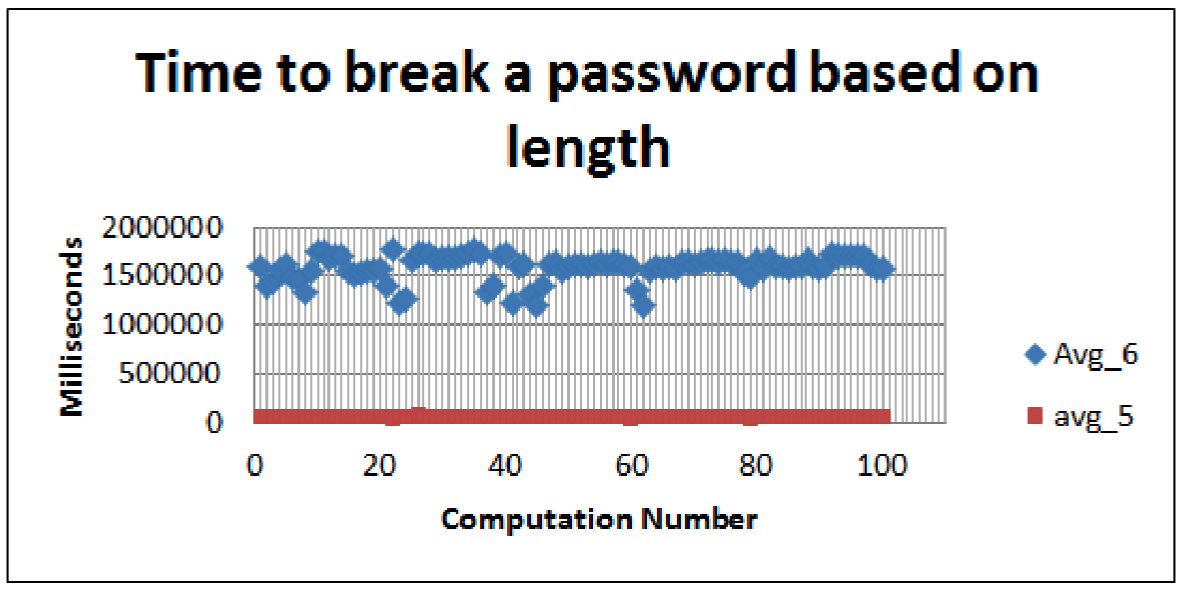
\includegraphics[width=0.7\textwidth]{img/abbildungen/length-time.png}
        \captionsetup{format=hang}
        \caption{Zeit, um ein Passwort zu brechen in Abhängigkeit zu der Länge} \label{timetobreak}
    \end{figure}

    Zwei Angriffsvektoren sind dabei zumeist betroffen: die Speicherung und der Mensch. Im Folgenden soll präziser erläutert werden, was diese beiden Angriffsvektoren so verwundbar machen:

    \textbf{Speicherung:}

    Viele Angreifer versuchen Passwörter zu kompromittieren, indem sie Zugriff auf die Datenbank erhalten, in welcher die Passwörter gespeichert sind. Mit Hilfe der erlangten Passwörtern erhoffen sie sich zumeist einen erweiterbaren Zugriff auf Systeme oder nutzen die Passwörter, um ihre Opfer zu erpressen \cite{boonkrong2012security}. Der wichtigste Faktor für den Erfolg solcher Angriffe spielt die Art der Speicherung. Abhängig von der Art wie Passwörter gespeichert sind offenbaren sich auch verschiedene Schwachstellen \cite{chanda2016password}.
    Die schlechteste, aber dennoch immer noch genutzte Art Passwörter zu speichern ist die Speicherung von Passwörtern im Klartext. Die Passwörter werden also in lesbarer Form gespeichert. Haben Angreifer also Zugriff auf die Datenbank, so können sie alle gespeicherten Passwörter ohne weiteren Aufwand auslesen \cite{chanda2016password}.

    Eine bessere Variante - allerdings weitaus nicht optimale - ist die Verschlüssellung der gespeicherten Passwörter. Der größte Kritikpunkt an dieser Variante ist allerdings, dass Verschlüssellungen zurückführbar sind. Das bedeutet mit dem Besitz des benötigten Schlüssels, lassen sich alle gespeicherten Daten ebenfalls in Klartext umwandeln. Hierbei müssen Angreifer also einen weiteren Aufwand erbringen, um an den benötigten Schlüssel zu gelangen. Sind sie allerdings im Besitz dieses Schlüssels können sie ebenfalls alle gespeicherten Passwörter auslesen \cite*{chanda2016password}. 

    Um die Sepicherung weiter zu optimieren sollte somit keine Zurückführbarkeit bestehen. Dies kann mit Hilfe von Hashing umgesetzt werden. Sog. Hashfunktionen erhalten einen Eingabewert und bilden diesen auf (im Optimalfall) einen einzigen Ausgabewert ab. Dieser Ausgabewert ist nicht zurückführbar auf den Eingabewert. Komprommittieren Angreifer also die Datenbank, in welcher die Passwörter gespeichert sind, können diese die gespeicherten Werte nicht direkt weiterverwenden. Auch dieser Ansatz birgt allerdings Schwachstellen. So lassen sich beispielsweise sog. Rainbow-Tables nutzen, um Hash-Werte zurückzuführen. Dies wird ermöglicht indem häufig genutzte Passwörter gehashed werden und dann mit Hash-Werten innerhalb der Datenbank verglichen werden \cite{chanda2016password}. 

    Um auch diese Schwachstelle zu verhindern, wird ein sog. Salt benötigt. Dabei wird an jedes Passwort, bevor es gehashed wird, ein individueller randomisierter Wert gehangen. Somit wird verhindert, dass sich der gespeicherte Hashwert mit Hilfe von Rainbow-Tables vergleichen lässt. Auch eine Umsetzung mit zwei Salt-Werten ist möglich. Dabei ist ein Salt öffentlich und der andere privat. So kann ebenfalls ein Schutz gegen offline-Angriffe geboten werden \cite{chanda2016password}.

\textbf{Faktor Mensch:}

Neben den aufgezählten technischen Aspekten, stellt der Mensch selbst eine der größten Angriffsvektoren bezogen auf Passwörter dar \cite{ives2004domino} \cite{yildirim2019encouraging}. Eins der größten Problem stellt der Aspekt dar, dass von Menschen erstellte Passwörter keine echten Zufallswerte sind. Das liegt insbesondere daran, dass Nutzer sich ihre Passwörter merken müssen. Je komplexer ein Passwort gestaltet ist, desto schwieriger wird es für Nutzer sich dieses zu merken - insbesonere, wenn sie sich mehrere verschiedene Passwörter merken müssen. Daher beinhalten Passwörter häufig Informationen, welche einen Bezug zum Inhaber haben. Dazu gehören Beispielsweise Namen, Geburtsdaten, Adressen, oder andere persönliche Informationen. Auch Passwörter, welche einfache Muster beinhalten sind sehr beliebt. Dazu gehören beispielsweise \textit{qwertz}, welches die ersten Buchstaben auf der Tastatur darstellt und \textit{123456}. Solche Passwörter können sich Menschen besser einprägen, was notwendig ist, wenn Passwörter häufig genutzt werden müssen. Aus dem identischen Grund neigen Nutzer ebenfalls dazu ein Passwort für mehrere Systeme zu nutzen \cite{chanda2016password} \cite{boonkrong2012security} \cite{yildirim2019encouraging}. 

Die genannten Faktoren führen dazu, dass die Anzahl an genutzten Kombinationen für ein Passwort deutlich geringer ist als die gesamte Menge an möglichen Kombinationen \cite{boonkrong2012security}. Das macht von Menschen erstellte Passwörter deutlich anfälliger für Angriffe, da diese einfacher zu erraten sind \cite{chanda2016password}. Dies liegt häufig auch daran, dass die Motivation der Nutzer häufig gering ist, komplexe Passwörter zu erstellen, weil sie sich der Gefahr von schwachen Passwörtern nicht bewusst sind \cite{yildirim2019encouraging}. Kontraproduktiv wirken in diesem Zusammenhang auch Policies und Richtlinien zur Erstellung von Passwörtern \cite{yildirim2019encouraging}. Sind die Richtlinien zur Erstellung von Passwörtern zu komplex, tendieren Nutzer bewusst dazu Muster in das Passwort einzubauen, um sich dieses zu merken. Dies führt zu einem gegenteiligen Effekt, da die Sicherheit und die Komplexität der Passwörter dadurch sinkt. Die These, dass solche Richtlininien zwangsweise zu einer erhöhten Sicherheit beitragen ist somit ein Irrglaube \cite{yildirim2019encouraging} \cite{morii2017research}.

Ein weiteres Problem stellt die die bereits genannte mehrfache Nutzung eines Passwortes für verschiedene Systeme dar. Aktive Internet-Nutzer verwalten im Durchschnitt 15 Passwörter pro Tag \cite{ives2004domino}. Um sich also das Einprägen verschiedener Passwörter zu ersparen, wählen Nutzer tendenziell lieber ein Passwort. Das führt häufig zu einem Domino-Effekt im Falle einer Passwort-Kompromittierung. Gelangen Angreifer an ein einzelnes Passwort des Nutzers, ist es häufig möglich mit diesem auch Zugriff auf andere Systeme zu gelangen \cite{ives2004domino} \cite{morii2017research}. 


\section{Passwortlose Authentifizierung} \label{alts}

Unter dem Sammelbegriff der passwortlosen Authentifizierung werden verschiedene Verfahren zusammengefasst, welche die Nutzung von Passwörten ersetzen sollen. Im Gegensatz zur passwortbasierten Authentifizierung steht also nicht mehr der Faktor \textit{something you know} im Vordergrund, da das Wissen des Nutzers nicht mehr die Grundlage zur Verifizierung seiner Identität darstellen soll. Die \ac{FIDO} Allianz nutzt den Begriff passwortlose Authentifizierung beispielsweise, um eine eine \ac{SFA} oder \ac{MFA} mit der Hilfe eines Security Keys zu beschreiben \cite{farke2020you}. 

Passwortlose Verfahren werden dabei als sicherer im Vergleich zur passwortbasierten Alternative angesehen, da viele der in \textbf{\ref{pw-auth}} aufgeführten Angriffsvektoren passwortlosen Ansätze nicht existieren \cite{chowhan2019password} \cite{parmar2022comprehensive}. Zudem erhofft man sich eine zusätzliche erhoffte Benutzerfreundlichkeit durch passwortlose Verfahren - insbesondere, weil Nutzer sich keine Passwörter mehr merken müssen und so ein geringerer Aufwand besteht \cite{chowhan2019password}.

Passwortlose Verfahren haben sich jedoch noch nicht flächendeckend durchgesetzt und sind nicht annähernd so weit verbreitet wie die Nutzung von Passwörtern. Dies lässt sich auf mehrere Faktoren zurückführen. Häufig genannte Gründe innerhalb der Fachliteratur sind die Umgewöhnung der Nutzer an eine neuartige Authentifizierung, welches als Hürde zur Etablierung der passwortlosen Verfahren angesehen wird. Aber auch zusätzliche entstehende Kosten durch die Integration der neuen Verfahren können eine Verbereitung ausbremsen \cite{chowhan2019password}. Ein detailierter Einblick in die Vor- und Nachteile in Bezug auf der Benutzerfreundlichkeit wird in \textbf{\ref{Yubikey}} gegeben.

Es gibt dabei eine Vielzahl an Möglichkeiten eine passwortlose AUthentifizierung umzusetzen. Eine der am häufigsten genutzen Varianten ist die Nutzung von Security Keys in Kombination mit FIDO2. Diese liegen im Fokus dieser Arbeit und werden in \textbf{\ref{Yubikey}} und \textbf{\ref{fido2}} genauer beschrieben. Dennoch sollen auch mögliche Alternativen kurz vorgestellt werden:


\begin{figure}[h]
	\centering 
	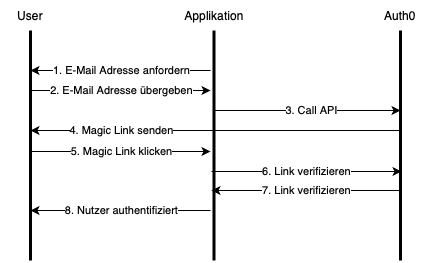
\includegraphics[width=0.7\textwidth]{img/abbildungen/magic_link.png}
	\captionsetup{format=hang}
	\caption{Beispielhafte Umsetzung eines Magic Links} \label{magiclink}
\end{figure}

\textbf{Magic Link:}

Bei einem Magic Link handelt es sich um eine
Authentifizierungsmöglichkeit, bei welcher Nutzer
lediglich ihren Benutzernamen oder ihre E-Mail-Adresse
zur Anmeldung angeben müssen. Anschließend erhält der Nutzer eine E-Mail mit einem dazugehörigen Link, welcher genutzt wird, um seine Identität zu verifizieren \cite{chowhan2019password} \cite{parmar2022comprehensive}.
Dieser Link beinhaltet einen Authentication Code, welcher im Hintergrund abgeglichen und validiert wird. Ist die Validierung erfolgreich wird der Nutzer authentifiziert und angemeldet. Nach der Anmeldung verliert der AUthentication Code seine Gültigkeit und somit auch der Link selbst \cite{chowhan2019password}. Der Ablauf des Verfahrens wird ebenfalls vereinfacht in \textbf{\ref{magiclink}} dargestellt.
Die Sicherheit dieses Verfahrens basiert dabei auf der Annahme, dass der Mail-Server bzw. der Zugang zum Account des Nutzers ausreichend geschützt ist. Ist diese Annahme nicht gegeben können sich auch andere Personen mit dem Link des eigentlichen Nutzers authentifizieren ohne autorisiert zu sein \cite{chowhan2019password}. 

\paragraph*{Vorteile:} Ein Passwort bleibt zwar in den meisten Fällen für den Zugriff auf den E-Mail Zugang notwendig, würde aber zumindest die Anzahl an benötigten Passwörtern für Nutzer reduzieren. Zudem handelt es sich bei einem Magic Link um eine sehr benutzerfreundliche und einfach verständliche Art der Authentifizierung \cite{parmar2022comprehensive}. Auch die Implementierung und die Kosten zur Instandshaltung sind verhältnismäßig gering einzuorden \cite{parmar2022comprehensive}.

\paragraph*{Nachteile:} Insbesondere im Unternehmenskontext kann die Nutzung von Spam-Filtern die Benutzerfreundlichkeit von Magic Links stark beeinträchtigen. So können beispielsweise die zugehörigen Mails fälschlicherweise als Spam klassifiziert werden oder eine erhöhte Wartezeit auf die E-Mail entstehen \cite{parmar2022comprehensive}. Auch im Bezug auf das Thema Sicherheit sind einige Aspekte fragwürdig. So hängt die Sicherheit des Verfahrens von der Sicherheit des Mail-Servers ab. Ist dieser nicht ausreichend geschützt, können Angreifer Zugriff auf die Mails erhalten und sich ebenfalls mit dem Link authentifizieren \cite{chowhan2019password}. Dies kann geschehen, ohne dass der Nutzer dies überhaupt bemerkt \cite{chowhan2019password}.

\textbf{\ac{OTP}:}

Das Konzept hinter \ac{OTP}s ähnelt dem des Magic Links. Nutzer geben ihre E-Mail-Adresse oder ihre Handynummer an (diese können ebenfalls einem Benutzernamen zugewiesen sein) und erhalten eine E-Mail/SMS, welche ein \ac{OTP} beinhaltet \cite{chowhan2019password} \cite{parmar2022comprehensive}. 
Dieses wird vom System abgeglichen und validiert. Ist die Validierung erfolgreich wird der Nutzer authentifiziert und angemeldet. Nach der Anmeldung verliert das \ac{OTP} seine Gültigkeit \cite{chowhan2019password}.
Häufig werden \ac{OTP}s allerdings nicht für eine oben beschrieben \ac{SFA} genutzt, sondern dienen als zusätzlicher Faktor für eine \ac{MFA} \cite{chowhan2019password}. So können beispielsweise Authenticator Apps zur Bereitstellung von \ac{OTP}s genutzt werden, um die etabliertere passwortbasierte Authentifizierung sicherer zu gestalten.
Im Gegensatz zu statischen, von Anwendern gewählten
Passwörtern sind \ac{OTP}s dynamisch erzeugt und haben nur
eine geringe Lebensdauer. So wird eine höhere
Sicherheit gewährleistet, da \ac{OTP}s nur schwierig durch
stupides Erraten oder Brute Force Attacken erbeutet
werden können \cite{chowhan2019password}.
Für die Umsetzung von OTPs gibt es mehrere Möglichkeiten. Zwei häufig verwendete Optionen sind \ac{HOTP} und \ac{TOTP} \cite{chowhan2019password}.
\ac{HOTP}s basieren auf der technischen Spezifikation RFC 4226. Sie werden mit Hilfe von \ac{HMAC} und unabhängig von der Zeit generiert. Neue \ac{HOTP}s können Event-basiert von dem Nutzer angefordert werden \cite{chowhan2019password}.
\ac{TOTP}s basieren auf der technischen Spezifikation RFC 6238 und werden in Abähngigkeit zu der Zeit erstellt. Sie ändern sich nach einem vordefinierten Zeitintervall und sind somit sehr kurzlebig \cite{chowhan2019password}.

\paragraph*{Vorteile:} Die Nutzung von \ac{OTP}s ist sehr effektiv für eine \ac{MFA}, da die Sicherheit im Vergleich zu einer passwortbasierten \ac{SFA} signifikant erhöht werden kann \cite{chowhan2019password} \cite{parmar2022comprehensive}. Zudem handelt es sich um eine sehr benutzerfreundliche und einfachz anwendbare Methode, welche sich bereits für die Nutzung von \ac{MFA} weitreichend etabliert hat \cite{parmar2022comprehensive}. Dies liegt auch an der Vielzahl an Umsetzungsmöglichkeiten von \ac{OTP}s, da diese beispielsweise via E-Mail, SMS, Authenticator App oder auch Security Key an den Nutzer übermittelt werden können \cite{chowhan2019password} \cite{parmar2022comprehensive}. 

\paragraph*{Nachteile:} Da sich diese Arbeit auf die Nutzung einer passwortlosen Authentifizierung als \ac{SFA} fokussiert, wird es hier als Nachteil eingeordnet, dass sich die Nutzung von \ac{OTP}s hauptsächlich für die Umsetzung einer \ac{MFA} anbietet. Eine Nutzung von \ac{OTP}s als \ac{SFA} wird häufig nicht unterstützt. Zudem ist je nach Implementierung wie auch bei einem Magic Link eine Abhängigkeit auf einen anderen Dienst gegeben, welche die Sicherheit des Verfahrens beeinträchtigen können.

\textbf{Biometrische Daten:}

Eine bereits weitreichend etablierte Methode zur passwortlosen AUthentifizierung ist die Nutzung von biometrischen Daten. Diese wird insbesondere im Bereich der mobilen Endgeräte häufig genutzt \cite{parmar2022comprehensive}. Dabei werden einzigartige biometrische Merkmale des Nutzers genutzt um seine Identität zu verifizieren. Dazu gehören beispielsweise Fingerabdrücke oder eine Gesichtserkennung \cite{parmar2022comprehensive}. Im Bereich der Smartphones wird dieses Beispielsweise von Apple durch die Technologien \textit{Touch ID} und \textit{Face ID} umgesetzt. Aber auch Microsoft bietet mittlerweile eine Authentifizierung mittels biometrischer Daten an (\textit{Windows Hello} und \textit{Hello for Business}). Diese Methode lässt sich ebenfalls für eine Integration in den Unternehmenskontext nutzen und ist nicht nur für mobile Endgeräte verfügbar. Wichtig ist hierbei, dass lediglich der reine Zugriff mit biometrischen Daten ermöglicht wird. Die Authentifizierung selbst basiert im Verlauf auf der Nutzung von öffentlich/privaten Schlüsselpaaren.

\paragraph*{Vorteile:} Viele mobile Endgeräte arbeiten bereits mit biometrischen Daten. Daher ist für eine Vielzahl an Nutzern keine große Umgewöhnung an die neue Art der Authentifizierung notwendig \cite{parmar2022comprehensive}. Da biometrische Daten nahezu einzigartig sind, sind diese ebenfalls deutlich schwieriger anzugreifen als Passwörter. Auch durch die Unterstützung von Microsoft über Windows Hello for Business ist diese Methode bereits für den Unternehmenskontext verfügbar \cite{parmar2022comprehensive}.

\paragraph*{Nachteile:} Äußere Bedingungen können die Erkennung von biometrischen Daten beeinträchtigen. So kann beispielsweise schlechtes Licht bei einer Gesichtserkennung oder staubige Umgebungen bei einem Fingerabdruckscanner die Erkennung beeinträchtigen \cite{parmar2022comprehensive}. Zudem können sich biometrische Daten im Laufe der Zeit verändern. Auch Verletzungen oder Krankheiten können zu Veränderungen der biometrischen Daten beitragen \cite{boonkrong2012security}. Auch wenn Microsoft bereits biometrische Daten unterstützt ist es im Unternehmenskontext häufig so, dass verschiedene Hersteller und Geräte genutzt werden. Diese unterstützen nicht alle biometrischen Daten oder sind nicht untereinander kompatibel \cite{parmar2022comprehensive}.

\textbf{Öffentliche/Private Schlüsselpaare:}

Bei der Nutzung von öffentlichen und privaten Schlüsselpaaren handelt es sich um eine asymmetrische Verschlüsselung. Dabei wird ein öffentlicher und ein privater Schlüssel generiert. Der öffentliche Schlüssel wird dabei an den Server übermittelt und der private Schlüssel wird auf dem Gerät des Nutzers gespeichert. Die AUthentifizierung erfolgt durch die Nutzung des privaten Schlüssels. Mit Hilfe des öffentlichen Schlüssels kann der Server die Identität des Nutzers verifizieren. Eine genaue Beschreibung des Verfahrens an Hand des FIDO2 Protokolls wird in \textbf{\ref{fido2}} gegeben.


\section{YubiKey} \label{Yubikey}
Ein Security Key ist eine Hardware, welche es ermöglicht einen Nutzer zu authentifizieren, indem dieser mit dem Security Key interagiert (beispielsweise durch einen Knopfdruck) \cite{reynolds2018tale}. In der Fachliteratur lassen sich viele verschiedene Bezeichnungen für Security Keys finden. Dazu gehören beispielsweise \textit{Security Token}, \textit{Hardware Token}, \textit{Authentifizierungsgerät}. Um eine einheitliche Bezeichnung zu gewährleisten, wird in dieser Arbeit der Begriff \textit{Security Key} genutzt. Beispielhaft wird in dieser Arbeit ein YubiKey der Series 5 (siehe \textbf{\ref{yubikey}}) als Referenzmodell genutzt. Dies basiert auf der Entscheidung, welche in \textbf{\ref{secwahl}} getroffen wird. Grundsätzlich sind die Funktionsweisen der verschiedenen Security Keys allerdings sehr ähnlich.

\begin{figure}[h]
	\centering 
	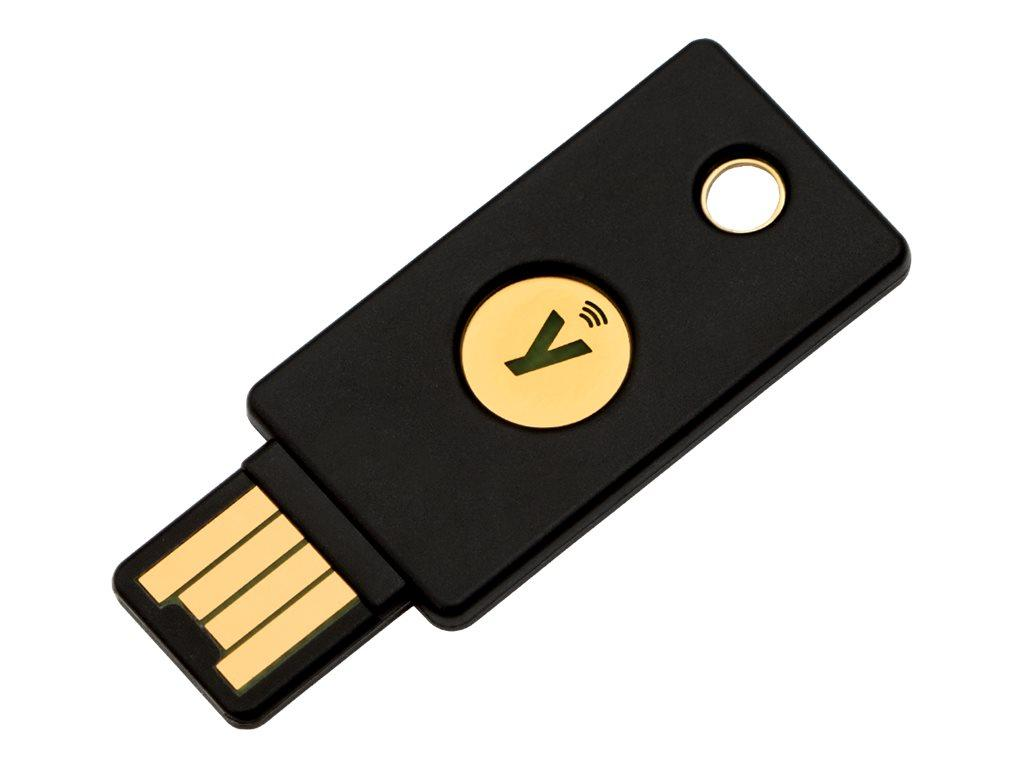
\includegraphics[width=0.3\textwidth]{img/abbildungen/yubikey.jpeg}
	\captionsetup{format=hang}
	\caption{Yubikey der Series 5} \label{yubikey}
\end{figure}

Der YubiKey 5 ermöglicht grundsätzlich drei Arten der Authentifizierung:

\begin{enumerate}
    \item Eine \ac{SFA}, welche Passwörter durch ein passwortloses \textit{tap-n-go} Verfahren ersetzt \cite{yuibkey2023fido2}.
    \item Eine Nutzung des Secruity Keys als zusätzlicher Faktor für eine \ac{2FA}. Somit wird das Passwort zusätzlich abgesichert. Der Security entspricht somit dem zweiten Faktor (\textit{something you have}) \cite{yuibkey2023fido2}.
    \item Eine passwortlose \ac{MFA} mit Hilfe einer zusätzlichen PIN für den Security Key \cite{yuibkey2023fido2}.
\end{enumerate}

\subsection{Usability}
Es gibt bereits Fachliteratur, welche sich mit der Benutzerfreundlichkeit von Security Keys beschäftigen. Diese beziehen sich zumeist auf die Implementierung von Security Keys in Kleinunternehmen. Die gesammelte Recherche soll genutzt werden um im Folgenden Vor- und Nachteile der Nutzung von Security Keys im Bezug auf deren Benutzerfreundlichkeit zu erläutern. Dies wird in \textbf{\ref{questions}} als Basis für die Evaluation eines Fragebogens für die \ac{LSY} genutzt.

\textbf{Vorteile:}

\begin{itemize}
    \item Ergebnisse zeigen, dass Nutzer grundsätzlich bereit sind, Passwörter durch passwortlose Verfahren zu ersetzen \cite{lyastani2020fido2}.
    \item Passwortlose Verfahren mit Security Key wurden mehr akzeptiert als tradionelle passwortbasierte Verfahren \cite{lyastani2020fido2}.
    \item Es handelt sich um eine implizite Garantie, dass sich lediglich Nutzer authentifizieren können, welche auch im Besitz des Security Keys sind \cite{lyastani2020fido2}.
    \item Durch die Nutzung von FIDO2 kann die Benutzerfreundlichkeit erhöht werden, da Nutzer sich keine Passwörter mehr merken müssen. Häufig wird das Verwalten der immer höher werdenden Anzahl an Passwörtern als Problem angesehen \cite{lyastani2020fido2} \cite{farke2020you}.
    \item Es wird ein deutlich geringerer kognitiver Aufwand benötigt, da Nutzer keine neuen Passwörter mehr erstellen und merken müssen \cite{lyastani2020fido2}.
    \item Zum aktuellen Zeitpunkt wird FIDO2 bereits von einer Vielzahl an Browsern unterstützt (und somit auch die Nutzung von Security Keys). Zusätzlich bieten immer mehr Online-Dienste die Möglichkeit an sich mit Hilfe von FIDO2 zu authentifizieren \cite{lyastani2020fido2} \cite{farke2020you}.
    \item Es handelt sich um offene und standardisierte Protokolle. Das verhindert verschieden Lösungsansätze verschiedener Hersteller und führt zu einer unabhängigeren und universellen Lösung \cite{farke2020you}.
\end{itemize}

\textbf{Nachteile:}

\begin{itemize}
    \item Im Falle einer \ac{SFA} wird der Verlust des Security Keys als größtes Problem angesehen. Bei Verlust hat auch der Nutzer keinen Zugriff mehr und aktuell gibt es noch keine sichere und effiziente Möglichkeiten, um den Zugriff wiederherzustellen \cite{lyastani2020fido2}.
    \item Da es sich um zusätzliche Hardware handelt kann diese ebenfalls kaputt gehen \cite{farke2020you}.
    \item Im Unternehmenskontext, kann die Verwaltung und Verteilung der Authentifizierungsgeräte zu einem Problem werden \cite{farke2020you}. 
    \item Da es sich um Hardware handelt, können Zugänge nicht an vertraute Personen weitergegeben werden, da der Zugang nur mit dem Authentifizierungsgerät möglich ist \cite{lyastani2020fido2}.
    \item Ohne das Authentifizierungsgerät sind keine spontanen Logins möglich \cite{lyastani2020fido2}.
    \item Bereits das aus der Tasche holen des Authentifizierungsgerätes ist für manche Nutzer bereits eine Hürde \cite{farke2020you}.
    \item Es wird ein physischer Aufwand benötigt, da das Authentifizierungsgerät mitgeführt werden muss \cite{lyastani2020fido2}.
    \item Authentifizierungsgeräte sind häufig mit Kosten verbunden, welche vom Nutzer getragen werden müssen \cite{lyastani2020fido2}.
    \item Nutzer haben Probleme ein neues Verfahren für die Authentifizierung zu nutzen, da sie sich an das alte Verfahren gewöhnt haben. Das führt dazu, dass Nutzer das neue Verfahren als kompliziert und ungewohnt empfinden. Sie verfügen häufig nicht über das nötige Wissen, um die Funktion und Sicherheit des Verafahrens zu verstehen \cite{lyastani2020fido2}.
    \item Selbst Nutzern, welchen das Konzept der passwortlosen Authentifizierung gefällt, nutzen in der Praxis häufig weiterhin Passwörter \cite{farke2020you}.
    \item Nutzer wollen keine Angewohnheiten verändern, wenn die nicht dazu gezwungen sind \cite{farke2020you}.
    \item Nutzer verwenden lieber Passwörter, da sie das Konzept und die Technologie besser verstehen \cite{lyastani2020fido2}.
    \item Nicht zwangsweise schneller als die Nutzung von Passwortmanagern \cite{farke2020you}.
    \item Allgemein fällt das Feeback von Nutzern weniger positiv aus, wenn diese vorher bereits Passwortmanager genutzt haben \cite{farke2020you}.
\end{itemize}

Insgesamt lassen sich noch nicht alle Szenarien mit Security Keys abdecken. Es gibt noch spezielle Fälle, in welchen die Nutzung von Passwörtern weiterhin notwendig ist \cite{lyastani2020fido2}. Auffälig jedoch ist, dass die Teilnehmer der Studien häufig einen skeptischen Blick auf die neuartige Authentifizierung werfen. Trotz der gesammelten Vor- und Nachteile kann keine Annahme darüber getroffen werden, ob die Vor- oder die Nachteile überwiegen und ob das Verfahren grundsätzlich gegenüber der passwortbasierten Alternative bevorzugt wird. Dies wird in \textbf{\ref{questions}} mit Hilfe der hier erarbeiteten Grundlage genauer analysiert.

\section{FIDO2} \label{fido2}

Es gibt bereits viele Alternativen zur passwortbasierten Authentifizierung. Einzelne wurden in \textbf{\ref{alts}} bereits beispielhaft beschrieben. Der Großteil dieser Alternativen wird allerdings nur in einem sehr geringen Ausmaß genutzt \cite{farke2020you}. \ac{FIDO}2 gehört zu den passwortlosen Verfahren, welche am meisten unterstützt werden. Das Protokoll wird von der \ac{FIDO} Allianz und dem \ac{W3C} entwickelt und bereitgestellt. Die \ac{FIDO} Allianz ist eine Organisation mit weltweit über 250 Mitgliedern. Darunter befinden sich Unternehmen wie Google, Microsoft, Apple, Amazon, Visa und viele mehr. Das \ac{W3C} wurde 1994 - mit dem Ziel das Wachstum des Internets zu gewährleisten - von Tim Berners-Lee gegründet. Es hat über 300 Mitglieder, darunter auch die hier aufgezählten Mitglieder der \ac{FIDO} Allianz  \cite{lyastani2020fido2} \cite{farke2020you} \cite{w3cabout}. Aus diesem Grund wird \ac{FIDO}2 von vielen Browsern standardmäßig unterstützt. Zudem gibt es eine Vielzahl an \ac{FIDO}2 kompatiblen Authentifizierungsgeräte, darunter u.A. Security Keys oder auch Smartphones \cite{lyastani2020fido2}.

Das Ziel bei der ENtwicklung von \ac{FIDO}2 ist es Nutzer zu authentifizieren, ohne dass diese ein Passwort verwenden müssen. Statt der Nutzung von Passwörtern basiert das Protokoll auf der Nutzung von Schlüsselpaareen. Dabei können Security Keys genutzt werden, aber auch das Gerät selber oder andere Authentifizierungsgeräte \cite{barbosa2021provable} \cite{morii2017research}. Diese können zusätzlich ebenfalls mit einer PIN oder biometrischen Daten abgesichert werden. Dabei ist die PIN nicht mit einem Passwort gleichzusetzen. Die PIN wird lediglich für das Authentifizierungsgerät genutzt und wird auch nur auf diesem gespeichert \cite{farke2020you} \cite{barbosa2021provable}. \ac{FIDO}2 unterstützt somit sowohl \ac{SFA} als auch \ac{MFA} \cite{lyastani2020fido2} \cite{farke2020you}. Zudem wird eine hohe Sicherheit ermöglicht, da Zugangsdaten bereitgestellt werden, welche nicht von Phishing oder Datenlecks betroffen sein können \cite{lyastani2020fido2}. Dies ist der Fall, da keine geteilten Geheimnisse zwischen Nutzer und Dienst existieren, welche auf einem Server gespeichert werden \cite{morii2017research}. 

\begin{figure}[h]
	\centering 
	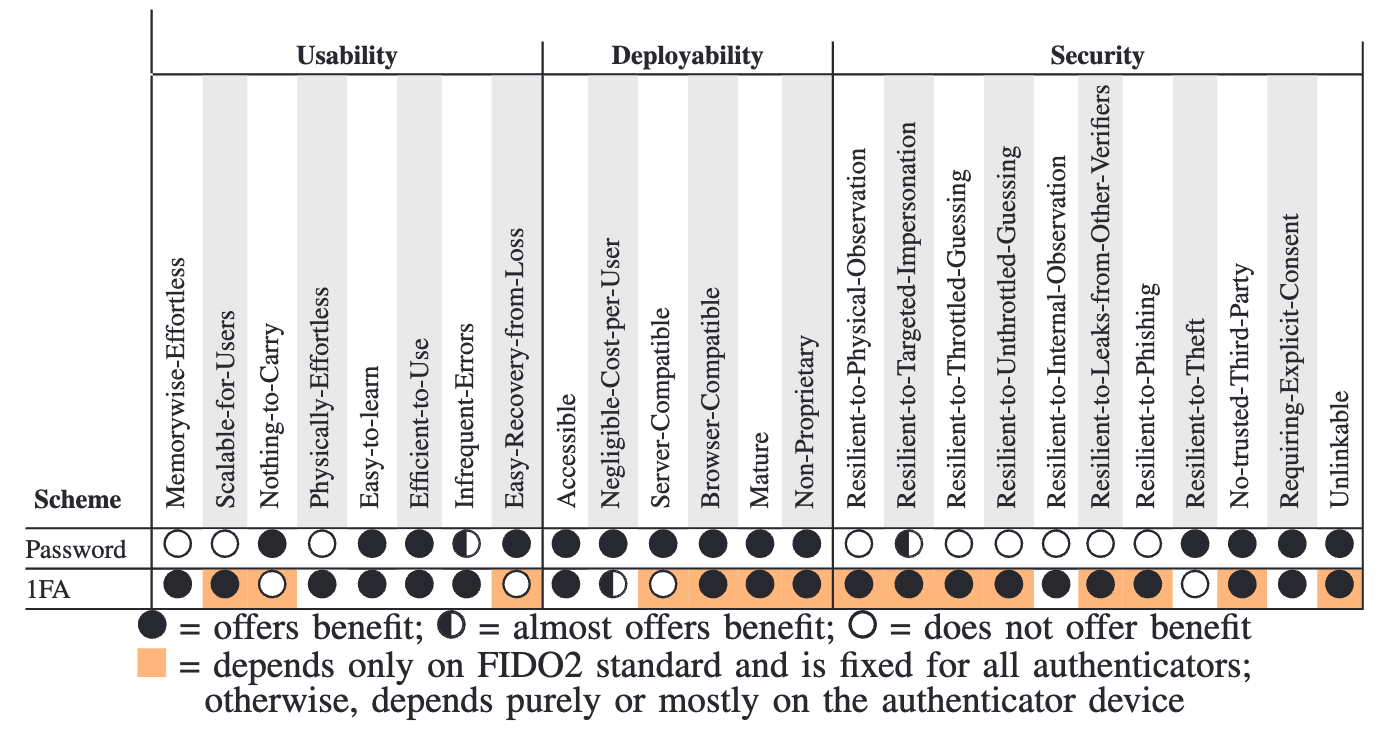
\includegraphics[width=1\textwidth]{img/abbildungen/fido2_usability.png}
	\captionsetup{format=hang}
	\caption{Mögliche Vorteile von FIDO2} \label{fido2-pros}
\end{figure}

In \textbf{\ref{fido2-pros}} werden die möglichen Vor- und Nachteile von \ac{FIDO}2 aufgezeigt. Dabei steht die Zeile \textit{1FA} für eine \ac{SFA} mit Hilfe von \ac{FIDO}2, welche mit der Nutzung von Passwörtern verglichen wird. Orange markiert in der \textit{1FA}-Zeile sind Bereiche, welche grundsätzlich von \ac{FIDO}2 abhängig sind. Weiß hinterlegte Bereiche sind zusätzlich abhängig vom genutzten Authentifizierungsgerät. Auffälig ist, dass insbesondere der Bereich \textit{Sicherheit} viele Vorteile bietet, welche grundsätzlich durch \ac{FIDO}2 ermöglicht werden und unabhängig vom genutzten Authentifizierungsgerät sind. Einige dieser Vorteile wurden bereits im Rahmen dieser Arbeit betrachtet. So lassen sich \ac{FIDO}2 Nutzerdaten beispielsweise nicht erraten oder phishen. Ebenfalls können diese nicht betroffen sein von Datenlecks und auch nicht durch Shoulder Surfing erlangt werden. Ein aufgezeigter Nachteil im Vergleich zu Passwörtern ist jedoch die Möglichkeit des Diebstahls eines Authentifizierungsgerätes. Dies ist allerdings abhängig vom genutzten Gerät und ergibt sich nicht durch die Nutzung von \ac{FIDO}2. Auch aufällig ist die große Abhängigkeit zum Authentifizierungsgerät im Bereich der Benutzerfreundlichkeit. Dort sind grundsätzlich zwar Vorteile gegenüber der Nutzung von Passwörtern möglich, aber nicht automatisch durch die Nutzung von \ac{FIDO}2 gegeben. 

\begin{figure}[h]
	\centering 
	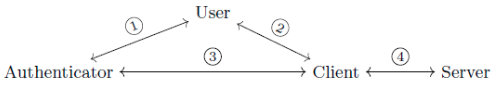
\includegraphics[width=0.8\textwidth]{img/abbildungen/fido2_com.png}
	\captionsetup{format=hang}
	\caption{FIDO2 Teilnehmer} \label{fido2-channels}
\end{figure}

Bei der Nutzung von \ac{FIDO}2 werden vier Kommunikationskanäle genutzt. Diese werden in \textbf{\ref{fido2-channels}} abgebildet. Es besteht eine Kommunikation zwischen User, Authentifizerungsgerät und dem Client. Der CLient ist üblicherweise ein Browser und übernimmt die Kommunikation mit dem Server. Vereinfacht wird der \ac{FIDO}2 Ablauf in \textbf{\ref{fido2-simple}} dargestellt. Der User meldet sich über den Client beim Server an (oder registriert sich erstmalig). Daraufhin sendet der Server eine Challenge an den Client weiter, welche vom Authentifizierungsgerät signiert werden muss. Der Client gibt die Challenge an das Authentifizierungsgerät weiter. Bevor dieser die Challenge signieren kann, muss der User die Aktion mit Hilfe einer Geste am Authentifizierungsgerät autorisieren (z.B. ein Knopfdruck). Anschließend signiert das Authentifizierungsgerät die Challenge und sendet diese an den Client zurück. Der Client sendet die signierte Challenge an den Server weiter. Der Server kann die Signatur mit Hilfe des öffentlichen Schlüssels verifizieren und den User authentifizieren \cite{lyastani2020fido2} \cite{farke2020you}. Dieser Ablauf wird im weiteren Verlauf genauer erläutert.

\begin{figure}[h]
	\centering 
	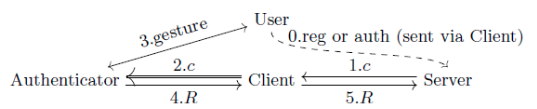
\includegraphics[width=0.8\textwidth]{img/abbildungen/fido2_flow.png}
	\captionsetup{format=hang}
	\caption{Vereinfachter FIDO2 Ablauf} \label{fido2-simple}
\end{figure}

Dieser aufgezeigte Ablauf besteht aus den zwei Subprotokollen \ac{CTAP2}, welches für die Kommunikation zwischen Client und Authentifizierungsgerät genutzt wird und WebAuthn, welches für die Kommunikation zwischen Client und Server zuständig ist. Dabei wird WebAuthn von dem \ac{W3C} spezifiziert und \ac{CTAP2} von der \ac{FIDO} Allianz \cite{farke2020you}.

\subsection{WebAuthn}
Bei WebAuthn handelt es sich um einen Standard, welcher es Webanwendungen ermöglicht Nutzer zu authentifizieren \cite{lyastani2020fido2}. Seit 2019 gehört WebAuthn zu den offiziellen Webstandards \cite{farke2020you}. Er spezifiziert eine standardiserte, vom Browser unabhängige JavaScript \ac{API} zur Authentifizierung von Nutzern für Webanwendungen. Ein großer Vorteil von WebAuth ist, dass es Webanwendungen ermöglicht wird eine Authentifizierung zu integrieren, welche resistent gegenüber Phsishing, Datenlecks und Passwortdiebstahl ist. Anstelle von geteilten Geheimnissen nutzt WebAuthn public-key Kryptographie, um einzigartige Zugangsdaten für jede Webanwendung zu erstellen, welche nur auf dem Gerät des Nutzers gespeichert werden \cite{farke2020you}. Es handelt sich dabei um ein sog. Challenge-Response-Verfahren zwischen einem Client und einem Server \cite{barbosa2021provable}. Die Sicherheit des Standards basiert auf dem Beweis, dass RSASSA PKCS1-v1\_5 und RSASSA-PSS als \ac{EUF-CMA} gelten und der Annahme, dass SHA-256 kollisionsresistent ist \cite{barbosa2021provable}.

WebAuthn unterstützt zwei Operationen: Registrierung und Anmeldung. In der Registrierungsphase sendet der Server dem Authentifizierungsgerät über den Client eine zufällige Challenge. In dieser Phase signiert das Authentifizierungsgerät mit Hilfe seines privaten Schlüssels die Challenge und sendet zusätzlich öffentliche Anmeldedaten für zukünftige Anmeldungen an den Server. Meldet sich ein bereits registrierter Nutzer an, wird die Challenge des Servers erneut von dem Authentifizierungsgerät signiert zurück an den Server gesendet. Der Server kann die Signatur mit Hilfe des öffentlichen Schlüssels verifizieren und den Nutzer authentifizieren \cite{barbosa2021provable}.

Dieser Prozess wird in \textbf{\ref{fido2-process}} genauer beschrieben (als schwarz dargestellt). Der Server \textit{S} sendet eine challenge message $m_{rch}$ über den Client $C$ an das Authentifizierungsgerät. Diese Challenge beinhaltet eine randomisierte Nonce, Parameter $UV$(beispielsweise, ob eine Nutzerverifizierung notwendig ist) und optional einen wert \textit{tb}, welcher den zugrunde liegenden Kanal eindeutig identifiziert (typischerweise eine \ac{TLS} Verbindung). Der Client $C$ erhält die challenge message $m_{rch}$ und wandelt diese in eine command message $m_{rcom}$ und eine client mesasage $m_{rcl}$ um. Die command message $m_{rcom}$ wird an das Authentifizierungsgerät $T$ übermittelt. Das Authentifizierungsgerät $T$ erzeugt ein öffentlich-privates Schlüsselpaar, welches an den Server $S$ gebunden ist und diesem ermöglicht, eine Verifizierung während der folgenden Authentifizierungsphase durchzuführen. Die erzeugten Daten werden dabei nur auf dem Authentifizierungsgerät $T$ gespeichert. Zudem gibt das Authentifizierungsgerät $T$ eine response message $m_{rrsp}$ aus. Der Client übergibt diese und die client message $m_{rcl}$ an den Server $S$. Die response message $m_{rrsp}$ beinhaltet einen \textit{attestation type}, welcher es dem Server $S$ ermöglicht eine Verifizierung während der Registrierungsphase durchzuführen und beinhaltet den öffentlichen Schlüssel. WebAuthn 2 unterstützt fünf \textit{attestation types}. Häufig werden die types \textit{None} und \textit{Basic} verwendet. Die restlichen types sind \textit{Self}, \textit{AttCA} und \textit{AnonCA}. \cite{bindel2022fido2}

Ist ein Nutzer bereits registriert, so empfängt der Client eine challenge message $m_{ach}$ von Server $S$ und wandelt diese in eine command message $m_{acom}$ und eine client message $m_{acl}$ um. Die command message $m_{acom}$ wird an das Authentifizierungsgerät $T$ übermittelt. Das Authentifizierungsgerät $T$ erzeugt eine response message $m_{arsp}$, welche mit dem privaten Schlüssel signiert wird und sendet diese an den Server $S$ (über den Client $C$). Der Server $S$ akzeptiert die response message $m_{arsp}$ und die client message $m_{acl}$ nur, wenn sie sich mit dem dazugehörigen öffentlichen Schlüssel und privaten Schlüssel des Servers $S$ verifizieren lassen. \cite{bindel2022fido2}

\begin{figure}[H]
	\centering 
	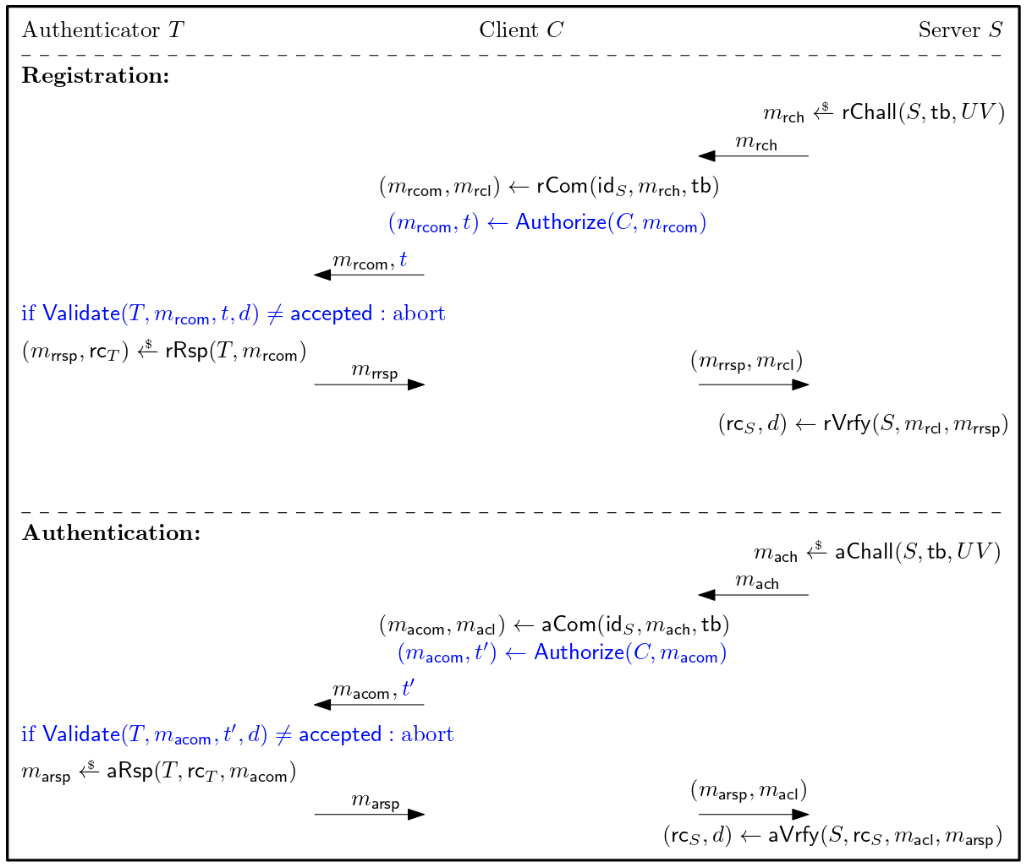
\includegraphics[width=1\textwidth]{img/abbildungen/Fido2.png}
	\captionsetup{format=hang}
	\caption{FIDO2 Darstellung} \label{fido2-process}
\end{figure}

\subsection{CTAP2}

\ac{CTAP2} wurde 2018 als internationaler Standard der \ac{ITU-T} anerkannt \cite{barbosa2021provable}. Es handelt sich um ein Protokoll auf der Anwendungsebene, welches für die Kommunikation zwischen eines WebAuthn Clients und eines konformen Authentifizierungsgerätes genutzt wird. Das Authentifizierungsgerät kann dabei ein externes Gerät sein, z.B. ein Security Key, welcher über USB, Bluetooth oder NFC eine Verbindung mit dem Client aufbaut. Aber auch interne Hardware eines Gerätes wie beispielsweise ein Fingerabdruckscanner oder ein Trusted Platform Module können als Authentifizierungsgerät genutzt werden \cite{lyastani2020fido2}.

Mit Hilfe von \ac{CTAP2} wird die Kommunikation zwischen einem Authentifizierungsgerät und einem Client spezifiziert. Der Client ist dabei üblicherweise ein Webbrowser. Das Ziel ist es zu garantieren, dass der Client das Authentifizierungsgerät nur nutzen darf, wenn der Nutzer dies autorisiert. Dafür muss der Nutzer beispielsweise einen Knopf am Authentifizierungsgerät drücken und/oder sich mit Hilfe eines PINs oder eines biometrischen Merkmals beim Authentifizierungsgerät authentifizieren. Das Ziel von \ac{CTAP2} ist es zunächst den Client an das Authentifizierungsgerät zu binden. Ist dies nicht der Fall, so wird es dem Client nicht ermöglicht sich zu authentifizieren. Dies wird auch in \textbf{\ref{fido2-process}} abgebildet. Die blauen Darstellungen betreffen den Prozess von \ac{CTAP2}. Bevor die command message $m_{rcom}$ an das Authentifizierungsgerät $T$ gelangt, muss der Nutzer mit Hilfe der persönlichen PIN $t$ die Aktion über den  Client $C$ autorisieren. Nach der Eingabe erfolgt die Übergabe an das Authentifizierungsgerät $T$, welcher diese validiert. Bei nicht erfolgreicher Validierung wird der Prozess abgebrochen \cite{barbosa2021provable}.

\ac{CTAP2} besteht dabei aus vier Phasen. Diese werden im Folgenden kurz erläutert. Da eine zu detailierte Beschreibung den Rahmen dieser Arbeit übertreffen würde, werden die Phasen lediglich in verinfachter Form erläutert. Eine detaillierte Darstellung ist \textbf{\ref{ctap2-process}} und wird genauer in \cite{barbosa2021provable} beschrieben. Folgende Phasen beinhaltet \ac{CTAP2}:

\begin{enumerate}
    \item In der Reboot Phase wird mit Hilfe eines unauthentifizierten \ac{ECDH} nach der NIST P-256 Spezifikation ein Schlüsselpaar $(a, aG)$ generiert (in \textbf{\ref{ctap2-process}} bezeichnet als ECKG). Zudem wird ein pinToken $pt$ erstellt und der mismatch counter $m$ auf den Wert drei gesetzt. Der mismatch counter $m$ wird genutzt, um die Anzahl der fehlgeschlagenen PIN Eingaben zu zählen \cite{barbosa2021provable}.  
    \item In der Setup Phase erfolgt ein unauthentifizierter \ac{ECDH} Schlüsselaustausch, gefolgt von der Übertragung des verschlüsselten PIN $c_p$ des Nutzers an das Authentifizierungsgerät $T$. Der geteilte Schlüssel $K$ für die Entschlüssellung ermittelt sich durch das Hashen der x-Koordinate $abG.x$ des \ac{ECDH}. Durch die Nutzung von AES-256-CBC $CBC_0$ und des Schlüssels $K$ lässt sich die PIN $c_p$ entschlüsseln. Diese wird vom Authentifizierungsgerät $T$ validiert. Ist die Validierung erfolgreich, wird Hash des PIN $pin_u$ als statisches Geheimnis $st_T.s$ lokal auf dem Authentifizierungsgerät $T$ gespeichert und der retries counter $st_T.n$ auf den standard Wert von acht gesetzt. Fallen diese acht Versuche fehl, so wird das Authentifizierungsgerät $T$ gesperrt \cite{barbosa2021provable} \cite{bindel2022fido2}.
    \item Die Bind Phase beginnt ebenfalls mit einem unauthentifizierten \ac{ECDH}. Darauf folgt eine Übertragung der erst gehashten und dann verschlüsselten PIN $c_{ph}$ vom Client $C$ an das Authentifizierungsgerät $T$. Diese wird vom AUthentifizierungsgerät $T$ entschlüsselt und mit dem statischen Geheimnis $st_T.s$ verglichen. Ist dieser Vergleich erfolgreich wird der pinToken $pt$ sowohl beim Authentifizerungsgerät $T$ als auch beim Client $C$ als binding state gesetzt \cite{barbosa2021provable} \cite{bindel2022fido2}.
    \item Zuletzt findet die Validierungs- und Autorisierungsphase statt. Der Client $C$ schickt einen Befehl mit einem HMAC Tag an das Authentifizerungsgerät $T$. Dieses validiert den Tag und autorisiert den Befehl nur, wenn eine \textit{positive decision} $d$ des Nutzers vorliegt (beispielsweise einem Knopfdruck) \cite{barbosa2021provable} \cite{bindel2022fido2}.
\end{enumerate}

Eine in der Fachliteratur häufig genannte Kritik an \ac{CTAP2} ist die Verwendung des unauthentifizierten \ac{ECDH}, welcher während der Binding und Setup Phase genutzt wird. Dieser kann von \ac{MITM} Angriffen betroffen sein \cite{barbosa2021provable}.
Zudem wird auch die Umsetzung der pinTokens kritisiert. Jedem Authentifizierungsgerät wird beim Hochfahren je ein pinToken zugeteilt. Das bedeutet mehrere Authentifizierungsgeräte können den gleichen pinToken besitzen. Dadurch wird die Sicherheit von \ac{CTAP2} limitiert \cite{barbosa2021provable}.

\begin{figure}[H]
	\centering 
	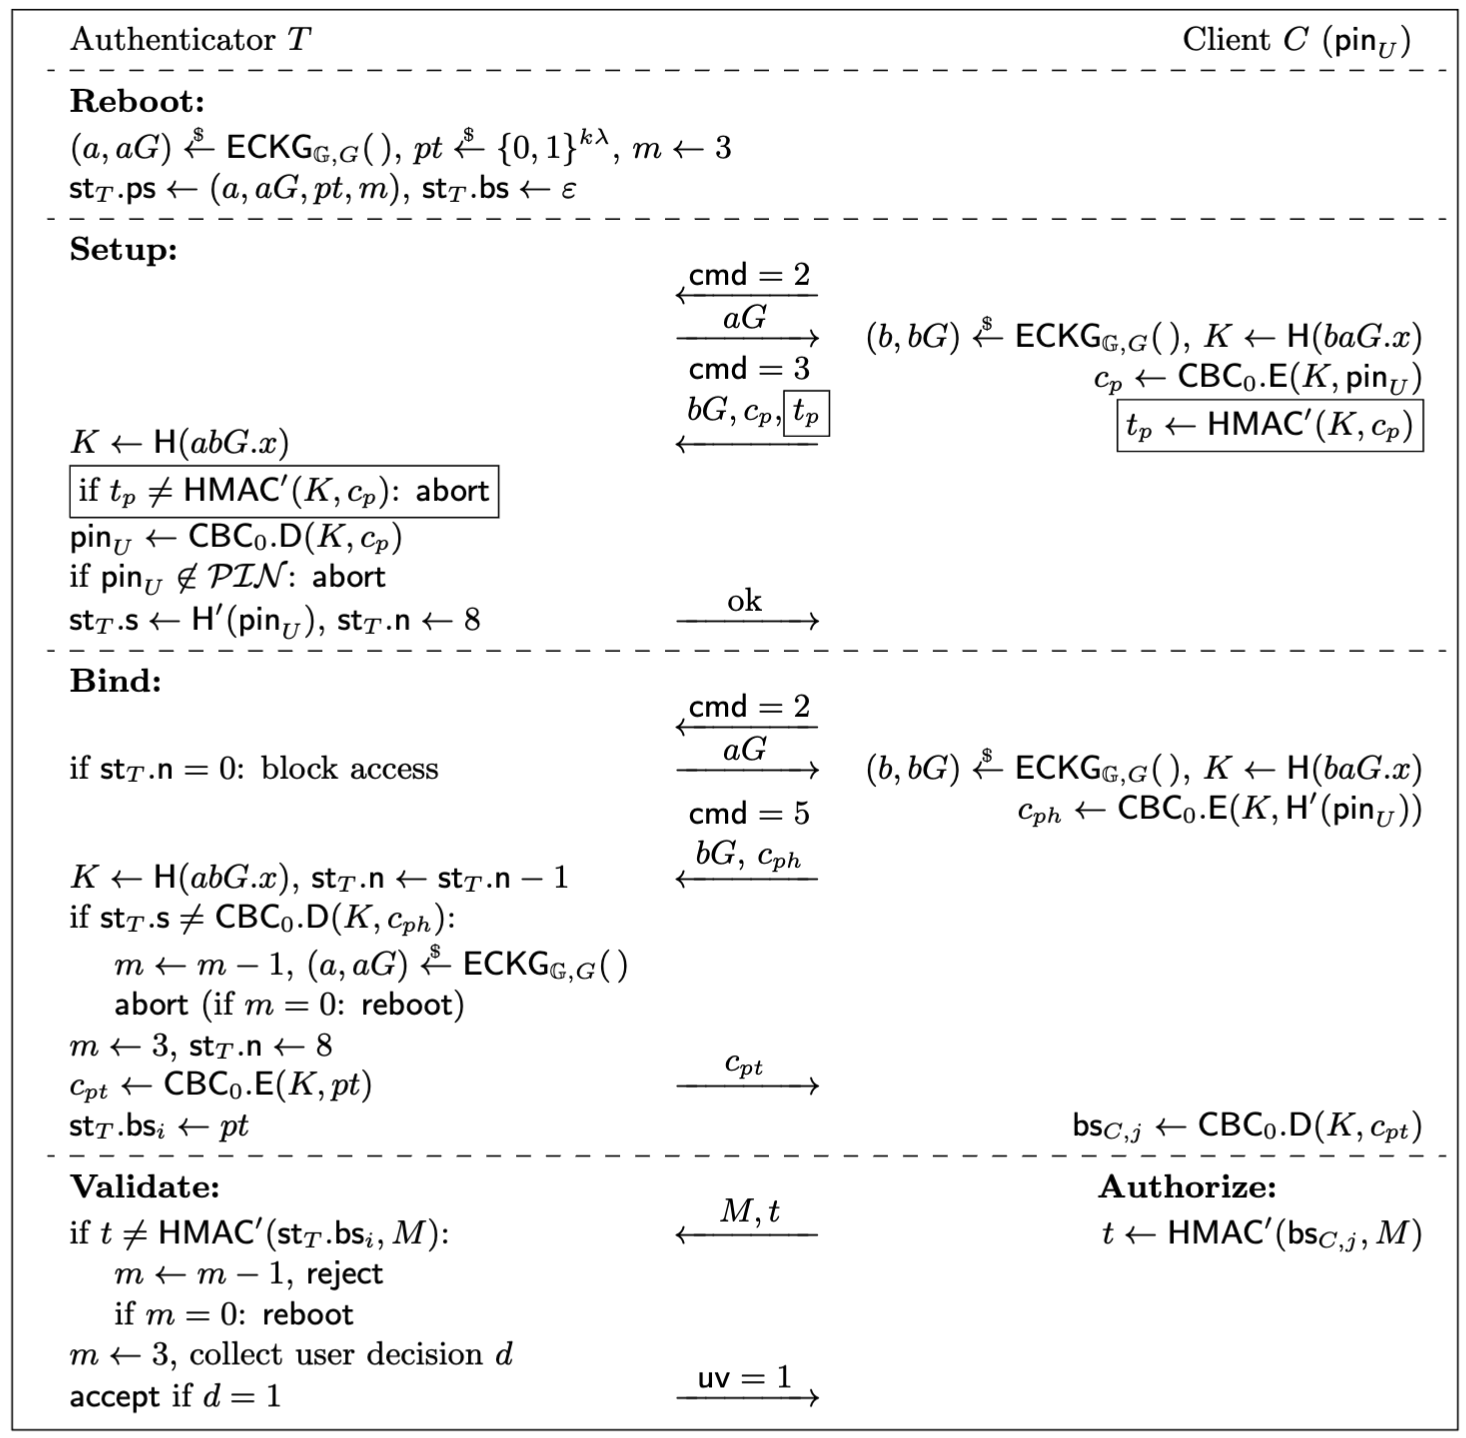
\includegraphics[width=1\textwidth]{img/abbildungen/ctap2-process.png}
	\captionsetup{format=hang}
	\caption{CTAP2} \label{ctap2-process}
\end{figure}

\subsubsection*{CTAP2.1}
Um diese Kritikpunkte zu beheben wurde CTAP2.1 entwickelt. CTAP2.1 basiert nicht mehr auf unauthentifizierten \ac{ECDH}, sondern auf einem sog. \ac{puvProtocol}. In Verbindung mit WebAuthn gilt CTAP2.1 als \ac{PQ} bereit, da ein Operationsmodus ermöglicht wird, welcher nur kryptographische Primitive und digitale Signaturen und \ac{KEM} verwendet \cite{bindel2022fido2}.

Zusätzlich werden die pinTokens im Vergleich zu \ac{CTAP2} anders erstellt. Während der pinToken bei \ac{CTAP2} aus mehreren 128 Bit-Blöcken besteht und keine maximale Begrenzung der Länge besitzt, wird der pinToken bei CTAP2.1 als pinUvAuthToken definiert. Dieser hat eine feste Länge von 128 oder 256 Bit. Der pinToken von \ac{CTAP2} wird bis zum nächsten Neustart wiederverwendet. Der pinUvAuthToken von CTAP2.1 wird nach jeder erfolgreichen Authentifizierung neu generiert. So besteht ein verringertes Risiko, dass sich mehrere Authentifizierungsgeräte den gleichen pinToken teilen. Das führt dazu, dass CTAP2.1 eine \ac{SUF}-t' Sicherheit aufweist und \ac{CTAP2} lediglich eine \ac{UF}-t' Sicherheit \cite{bindel2022fido2}. Ebenfalls ermöglicht CTAP2.1 die Nutzung von biometrischen Merkmalen, anstelle von einer individuellen PIN \cite{bindel2022fido2}.


\subsection{Sicherheit}

\ac{FIDO}2 wird in der Fachliteratur als grundsätzlich sicheres Protokoll angesehen. Es ist eine Erweiterung des \ac{FIDO} \ac{U2F} Protokolls und es handelt sich um geprüfte asymmetrische Kryptographie \cite{lyastani2020fido2} \cite{farke2020you}. Im Folgenden sollen kurz die wichtigsten Vorteile im Aspekt der Sicherheit aufgezeigt werden:


\begin{itemize}
    \item Es gibt keine geteilten Geheimnisse zwischen Usern und Diensten, welche durch Phishing oder Datenlecks kompromittiert werden können \cite{lyastani2020fido2} \cite{farke2020you}. 
    \item Dasas selbe Authentifizierungsgerät für mehrere Dienste nutzbar, ohne dass sich dabei eine Verknüpfung zurückführen lässt \cite{lyastani2020fido2} \cite{farke2020you}.
    \item es kann lediglich die Session kompromittiert werden und nicht die Zugangsdaten selbst \cite{morii2017research}.
    \item Authentifizierungsgeräte lassen sich mit zusätzlichen PINs oder biometrischen Merkmalen absichern, um sich ebenfalls vor Diebstahl schützen \cite{barbosa2021provable}.
    \item Zugangsdaten können nicht durch systematisches erraten kompromittiert werden \cite{barbosa2021provable}.
    \item Wird ein Security Key gestohlen, kann dieser nur genutzt werden, wenn ebenfalls der PIN bekannt ist \cite{barbosa2021provable}.
\end{itemize}

In folgendem Szenario:

\begin{enumerate}
    \item Der Nutzer besitzt ein Authentifizierungsgerät, welcher mit einem drückbaren Knopf oder ähnlichen ausgestattet ist.
    \item Das Authentifizierungsgerät ist mit einem geheimen PIN oder biometrischen Merkmalen geschützt.
    \item Der Nutzer autorisiert vertrauten Clients auf das Authentifizierungsgerät zuzugreifen.
    \item Der Nutzer verbindet sein Authentifizierungsgerät mit mehreren Clients und nutzt diese um sich bei mehreren Webdiensten zu registrieren/anzumelden.
\end{enumerate}

Dann ist versichert, dass:

\begin{enumerate}
    \item Die Authentifizierung von dem Authentifizierungsgerät durchgeführt wurde, welcher die genutzen Zugangsdaten bei dem Webdienst registriert hat.
    \item Ein autorisierter Befehl auf das Authentifizierungsgerät zugegriffen hat.
    \item Dieser autorisierte Befehl von einem autorisierten Client beauftragt wurde (sollte der Nutzer den korrekten PIN eingegeben haben).
\end{enumerate}

Unter der Voraussetzung, dass:

\begin{enumerate}
    \item Das Authentifizierungsgerät nicht gestohlen wurde.
    \item Der PIN des Authentifizierungsgerätes nicht kompromittiert wurde.
    \item Der autorisierte Client nicht kompromittiert wurde (korrekte Ausführung von \ac{CTAP2} und Client ist nicht von böswilliger Software betroffen).
\end{enumerate}

